{\fontsize{12}{14}\selectfont 

\begin{figure}[H]
  \centering
  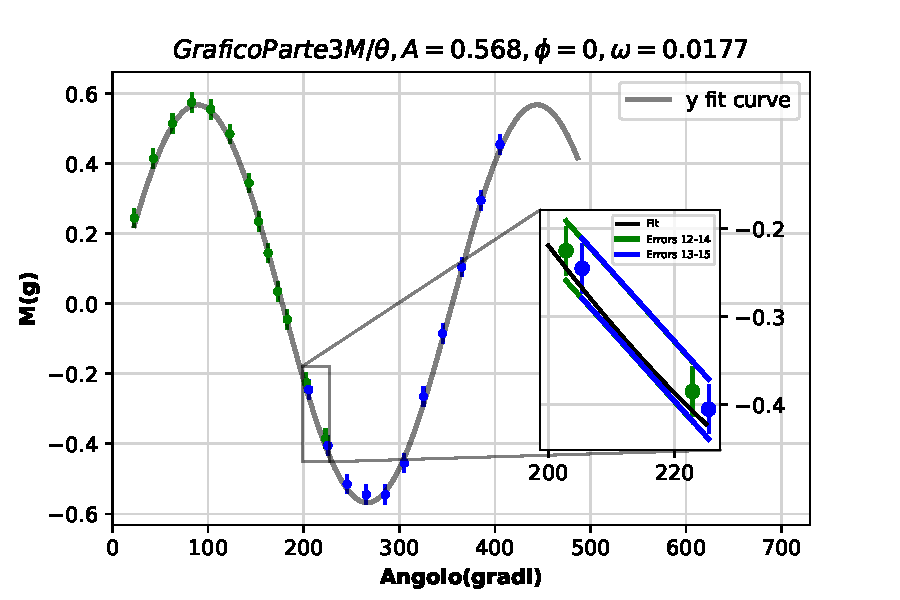
\includegraphics[width=15cm]{Figures/GraficoMthetaParte3.pdf}
  \caption{Grafico della differenza di massa in grammi in funzione dell'angolo $\theta$ in gradi. La variazione di massa è stata ottenuta come differenza con la massa a circuito aperto e gli è stato attribuito un errore di $0.02g$ ottenuto da una somma diretta degli errori sulle singole pesate. Le misure sono state prese facendo ruotare il circuito dell'\emph{accessory unit} a corrente fissata di 1A. Per l'errore sull'angolo è stata presa mezza tacca sul goniometro, ovvero 0.5°.
  Si nota un andamento sinusoidale compatibilmente con la formula [\ref{eq:FL}].}   
  \label{fig:GraficoParteIII}
\end{figure}
I valori di ampiezza, fase e frequenza sono stati ricavati dal fit $M = A \cdot sin(\omega \cdot t + \phi)$; l'errore di ciascun parametro è stato stimato variando manualmente il suo valore in modo che la curva rientrasse nelle barre di errore dei dati.

\begin{equation*}
    A = (0.568 \pm 0.005) g \qquad \phi = (0.00 \pm 0.02) \text{rad} \qquad \omega = (0.01768 \pm 0.00008)\text{rad}/s %review
\end{equation*}

\par}